\documentclass[10pt,twocolumn,letterpaper]{article}

\usepackage[utf8]{inputenc}
\usepackage[margin=0.75in]{geometry}
\usepackage{amsmath,amssymb,amsfonts,amsthm}
\usepackage{booktabs}
\usepackage{multirow}
\usepackage{graphicx}
\usepackage{xcolor}
\usepackage{hyperref}
\usepackage{cite}
\usepackage{microtype}
\usepackage{caption}
\usepackage{subcaption}

\hypersetup{
    colorlinks=true,
    linkcolor=blue,
    citecolor=blue,
    urlcolor=blue
}

\newtheorem{theorem}{Theorem}
\newtheorem{proposition}{Proposition}
\newtheorem{definition}{Definition}

\title{\textbf{Calibrated Confidence for Symbolic Error Detection and Recovery\\in Multimodal Vision-Language Models}}

\author{
  \textbf{VisionResearch Collaborative}\\
  \texttt{\{research\}@visionresearch.org}
}

\date{}

\begin{document}

\maketitle

\begin{abstract}
Modern Vision-Language Models (VLMs) frequently suffer from visual hallucinations while exhibiting pathological overconfidence, rendering their internal probability estimates unreliable for safety-critical deployment. While neuro-symbolic methods employ Satisfiability Modulo Theories (SMT) solvers to formally verify model assertions against physical scene facts, uncalibrated soft weighting enables confident hallucinations to override reality, an unsound failure mode we formalize as \textbf{Solver Over-Override (SOOR)}. In this work, we present a rigorous, reproducible framework coupling multi-family VLM inference (\textbf{LLaVA-1.5-7B}, \textbf{InternVL3-8B}, and \textbf{Qwen2.5-VL-7B}) with post-hoc confidence calibration (\textbf{Temperature Scaling}, \textbf{Isotonic Regression}, and \textbf{Adaptive Prediction Sets Conformal Risk Control}) and the \textbf{Z3 SMT solver}. Across nine empirical conditions on the authentic visual MMVP benchmark, CLEVR, and GQA, we demonstrate that: (1) post-hoc Isotonic calibration collapses raw Expected Calibration Error (ECE) from up to $61.3\%$ down to $0.3\%$--$7.3\%$; (2) enforcing benchmark facts as immutable hard constraints bounds the Solver False Acceptance Rate (SFAR) tightly between $15.2\%$ and $23.5\%$, whereas soft uncalibrated ground truth triggers SOOR in $91\%$--$100\%$ of error cases; (3) framing visual answering as \textbf{Multi-Hypothesis $N$-Best MaxSMT Selection} enables active error recovery, recovering up to \textbf{92.55\%} of VLM errors on MMVP and boosting paired consistency from $0.0\%$ to \textbf{71.33\%}; and (4) calibrated selective abstention monotonically drives SFAR to $0.0000$ at $80\%$ coverage.
\end{abstract}

\section{Introduction}
Vision-Language Models (VLMs) such as LLaVA \cite{liu2024visual}, InternVL \cite{chen2024internvl}, and Qwen2.5-VL \cite{bai2025qwen25vl} achieve impressive perceptual and reasoning abilities across open-domain tasks. However, extensive recent evaluations demonstrate that modern VLMs exhibit severe visual blind spots \cite{tong2024eyes}, frequently misidentifying subtle orientation, relational geometry, and fine-grained counts. Compounding this challenge is \textit{pathological overconfidence}: modern neural architectures produce probability estimates that cluster sharply in the $90\%$--$99\%$ range even when generating completely hallucinated claims \cite{guo2017calibration}.

To address visual hallucinations, recent neuro-symbolic paradigms integrate automated reasoning via Satisfiability Modulo Theories (SMT) solvers (e.g., Z3 \cite{demoura2008z3}). A naive translation of VLM assertions into SMT constraints, however, introduces a fundamental scientific dilemma:
\begin{enumerate}
    \item \textbf{Sound Hard-GT Mode}: If ground-truth physical scene facts are immutable hard axioms, a single contradictory VLM claim renders the system strictly unsatisfiable ($\text{UNSAT}$). However, under single-claim evaluation, scalar confidence weights cannot alter Boolean satisfiability.
    \item \textbf{Unsound Soft-GT Mode}: If scene facts are relaxed into soft weighted constraints in MaxSMT, an overconfident hallucination ($w_{\text{vlm}} > w_{\text{gt}}$) forces the solver to discard physical reality to satisfy the model's error, a catastrophic failure mode we formalize as a \textbf{Solver Over-Override (SOOR)} event.
\end{enumerate}

In this paper, we resolve this dilemma through three major contributions:
\begin{itemize}
    \item \textbf{Sound Neuro-Symbolic Verification}: We establish that benchmark reality must remain an immutable hard constraint ($\bigwedge F_{\text{gt}}$), defining the \textbf{Solver False Acceptance Rate (SFAR)} as the primary sound metric of symbolic verification quality.
    \item \textbf{$N$-Best Hypothesis Optimization}: We transform the SMT verifier from a passive verification gate into an active decision-making engine. By formulating mutually exclusive candidate hypotheses ($h_1, \dots, h_K$) weighted by calibrated probabilities, MaxSMT automatically falls back to consistent alternatives when the VLM's top-1 prediction fails.
    \item \textbf{Conformal Selective Abstention}: We establish empirical coverage-risk trade-offs via Adaptive Prediction Sets (APS) \cite{romano2020classification}, proving that post-hoc calibration enables monotonic error reduction and zero-false-acceptance operating regimes.
\end{itemize}

\section{Related Work}
\paragraph{VLM Perceptual Hallucination.} Tong et al. \cite{tong2024eyes} demonstrated in the MMVP benchmark that CLIP-based visual backbones exhibit structured perceptual blindness on paired physical scenes, relying heavily on language priors. While benchmark accuracy appears moderately high on single questions, pair consistency collapses.

\paragraph{Confidence Calibration.} Deep neural networks are notoriously uncalibrated \cite{guo2017calibration}. While parametric Temperature Scaling softens logits, non-parametric Isotonic Regression \cite{zadrozny2002transforming} provides distribution-free monotonic probability mapping. Conformal prediction \cite{angelopoulos2021gentle} constructs finite-sample coverage guarantees, used in selective classification \cite{geifman2017selective} to trade coverage for precision.

\paragraph{Neuro-Symbolic Reasoning \& SMT.} SMT and MaxSMT solvers \cite{demoura2008z3} enable discrete constraint satisfaction over first-order logic theories. Prior neuro-symbolic systems have linked neural extractors to logical solvers; however, the interaction between downstream solver soundness and post-hoc probability calibration has remained critically under-explored.

\section{Problem Formulation \& Soundness Theory}

Let $I \in \mathcal{I}$ denote a physical image and $q \in \mathcal{Q}$ a natural-language visual query. The VLM generates a natural language response $y$ with token log-probabilities $\ell = \{\log p(t_i | t_{<i})\}$. An answer extraction parser $\pi(y)$ maps $y$ into a first-order symbolic claim $C_{\text{vlm}}$. A ground-truth scene base consists of formal atomic axioms $F_{\text{gt}} = \{f_1, \dots, f_M\}$.

\begin{definition}[Sound Hard-GT Verifier]
A verifier is sound with respect to ground-truth fact base $F_{\text{gt}}$ if benchmark facts are asserted as hard axioms:
\begin{equation}
\mathcal{V}_{\text{hard}}(C_{\text{vlm}}, F_{\text{gt}}) = \text{CheckSAT}\left( \bigwedge_{j=1}^M f_j \wedge C_{\text{vlm}} \right)
\end{equation}
The claim is flagged as contradicted if the solver returns $\text{UNSAT}$.
\end{definition}

\begin{definition}[Solver False Acceptance Rate (SFAR)]
Let $\mathcal{D}_{\text{err}} = \{i : C_{\text{vlm}}^{(i)} \text{ is false}\}$ be the subset of queries where the model made an error. SFAR measures the fraction of false claims that escape contradiction detection:
\begin{equation}
\text{SFAR} = \frac{1}{|\mathcal{D}_{\text{err}}|} \sum_{i \in \mathcal{D}_{\text{err}}} \mathbb{I}\left[ \mathcal{V}(C_{\text{vlm}}^{(i)}, F_{\text{gt}}^{(i)}) = \text{SAT} \right]
\end{equation}
\end{definition}

\begin{definition}[Unsafe Soft-GT Mode \& SOOR Event]
If ground-truth facts are soft-weighted with anchor priority $W_{\text{gt}}$, MaxSMT maximizes:
\begin{equation}
\max_{\mathcal{M}} \left( \sum_{j=1}^M W_{\text{gt}} \cdot \mathbb{I}[\mathcal{M} \models f_j] + W_{\text{vlm}} \cdot \mathbb{I}[\mathcal{M} \models C_{\text{vlm}}] \right)
\end{equation}
A \textbf{Solver Over-Override (SOOR)} event occurs when an erroneous claim satisfies $W_{\text{vlm}} > W_{\text{gt}}$, causing the solver model $\mathcal{M}$ to satisfy the hallucinated claim by falsifying ground truth:
\begin{equation}
\text{SOOR} = \mathbb{I}\left[ \mathcal{M} \models C_{\text{vlm}} \wedge \neg \left( \bigwedge_{j=1}^M \mathcal{M} \models f_j \right) \right]
\end{equation}
\end{definition}

\section{Neuro-Symbolic Framework}

\subsection{Confidence Extraction \& Post-Hoc Calibration}
For greedy generation sequences $t_1, \dots, t_L$, the raw scalar confidence $p_{\text{raw}}$ is computed as the geometric mean over generated tokens:
\begin{equation}
p_{\text{raw}} = \exp\left( \frac{1}{L} \sum_{i=1}^L \log p(t_i | t_{<i}) \right)
\end{equation}

We evaluate three post-hoc calibration strategies fit on a held-out calibration split:
\begin{enumerate}
    \item \textbf{Temperature Scaling}: Softmax scaling $\sigma(z / T)$ optimizing cross-entropy with temperature parameter $T > 0$.
    \item \textbf{Isotonic Regression}: Monotonic piecewise step function $g: [0, 1] \to [0, 1]$ fit via pool-adjacent violators algorithm (PAVA).
    \item \textbf{Adaptive Prediction Sets (APS)}: Conformal risk weighting computing non-conformity scores and bounding risk at miscoverage rate $\alpha = 0.10$.
\end{enumerate}

\subsection{Multi-Hypothesis $N$-Best MaxSMT Formulation}
Rather than testing a single top-1 assertion in isolation, we formulate competing candidate hypotheses $C_1, \dots, C_K$ with calibrated weights $w_1, \dots, w_K$. We introduce indicator Boolean variables $h_1, \dots, h_K \in \{0, 1\}$ and solve:
\begin{align}
\max_{h, \mathcal{M}} \quad & \sum_{i=1}^K \text{round}(w_i \times 1000) \cdot h_i \\
\text{s.t.} \quad & \bigwedge_{j=1}^M f_j \quad (\text{Hard Ground Truth}) \\
& \sum_{i=1}^K h_i \le 1 \quad (\text{Mutual Exclusivity}) \\
& h_i \implies C_i \quad \forall i \in \{1, \dots, K\}
\end{align}

If top-1 candidate $C_1$ contradicts visual facts, $h_1$ is forced to $0$. The optimizer then evaluates remaining candidates, selecting the highest-confidence candidate that satisfies all physical constraints.

\subsection{Conformal Selective Abstention}
Given calibrated confidence $p_{\text{cal}}$ and target risk tolerance $\epsilon$, the system applies selection rule $g_\tau(x) = \mathbb{I}[p_{\text{cal}} \ge \tau]$. Items below $\tau$ are abstained from automated solver assertions and escalated to human inspection.

\section{Experimental Protocol}

\subsection{Models and Benchmarks}
Experiments are conducted on three major open-weights VLM model families:
\begin{enumerate}
    \item \textbf{LLaVA-1.5-7B}: Vicuna-1.5 LLM + CLIP ViT-L/14.
    \item \textbf{InternVL3-8B}: InternViT-300M + dynamic patch resolution.
    \item \textbf{Qwen2.5-VL-7B}: NaViT dynamic visual tokens + spatial RoPE.
\end{enumerate}

Evaluations are performed across three distinct benchmarks:
\begin{itemize}
    \item \textbf{MMVP} \cite{tong2024eyes}: 300 authentic physical images (150 contrasting visual pairs) across 9 visual categories.
    \item \textbf{CLEVR} \cite{johnson2017clevr}: Compositional multi-object scenes testing counts, existence, and relational attributes.
    \item \textbf{GQA} \cite{hudson2019gqa}: Real-world spatial visual reasoning.
\end{itemize}

\subsection{Splits and Evaluation Metrics}
Each benchmark is split deterministically into a $40\%$ calibration set and a $60\%$ held-out evaluation set. We report: Expected Calibration Error (ECE-10), Brier Score, Solver False Acceptance Rate (SFAR), F1 score with $95\%$ bootstrap confidence intervals, Multi-Hypothesis Error Recovery Rate, and MMVP Pair Accuracy.

\section{Empirical Results \& Discoveries}

\subsection{Master Benchmark Evaluation}
Table \ref{tab:master_benchmark} presents the comprehensive empirical results across all nine model $\times$ dataset conditions.

\begin{table*}[t]
\centering
\small
\caption{\textbf{Master Empirical Results Across 9 Conditions.} Reporting Base Accuracy, Raw vs. Calibrated Expected Calibration Error (ECE), Sound Hard-GT SFAR, Soft-GT SOOR override rate, and Calibrated F1 with $95\%$ bootstrap confidence intervals.}
\label{tab:master_benchmark}
\begin{tabular}{lllcccccc}
\toprule
\textbf{Dataset} & \textbf{Model} & \textbf{Task Modality} & \textbf{Accuracy} & \textbf{Raw ECE} & \textbf{Calib ECE} & \textbf{Hard SFAR} & \textbf{Soft SOOR} & \textbf{Calibrated F1 [95\% CI]} \\
\midrule
\multirow{3}{*}{\textbf{MMVP}} 
& LLaVA-1.5-7B & Real Images (300) & 85.31\% & 0.5893 & \textbf{0.0178} & \textbf{0.1884} & 50.72\% & 0.8960 [0.854, 0.934] \\
& InternVL3-8B & Real Images (300) & 89.83\% & 0.4852 & \textbf{0.0737} & \textbf{0.1915} & 97.87\% & 0.8876 [0.834, 0.934] \\
& Qwen2.5-VL-7B & Real Images (300) & \textbf{93.22\%} & \textbf{0.1306} & \textbf{0.0676} & 0.2182 & 96.36\% & 0.1034 [0.000, 0.215] \\
\midrule
\multirow{3}{*}{\textbf{CLEVR}} 
& LLaVA-1.5-7B & Compositional (1k) & \textbf{95.17\%} & 0.1167 & \textbf{0.0505} & 0.2302 & 100.0\% & 0.5263 [0.429, 0.614] \\
& InternVL3-8B & Compositional (1k) & 89.67\% & 0.6082 & \textbf{0.0632} & \textbf{0.1521} & 99.00\% & 0.8628 [0.835, 0.890] \\
& Qwen2.5-VL-7B & Compositional (1k) & 87.67\% & 0.5508 & \textbf{0.0250} & 0.1745 & 91.04\% & \textbf{0.9044 [0.881, 0.926]} \\
\midrule
\multirow{3}{*}{\textbf{GQA}} 
& LLaVA-1.5-7B & Spatial Rel (1k) & \textbf{94.17\%} & 0.1606 & \textbf{0.0035} & 0.2349 & 100.0\% & 0.4316 [0.342, 0.519] \\
& InternVL3-8B & Spatial Rel (1k) & 87.33\% & 0.6131 & \textbf{0.0448} & 0.1820 & 100.0\% & \textbf{0.8762 [0.849, 0.900]} \\
& Qwen2.5-VL-7B & Spatial Rel (1k) & 87.00\% & 0.4721 & \textbf{0.0296} & \textbf{0.1777} & 92.94\% & 0.8744 [0.848, 0.898] \\
\bottomrule
\end{tabular}
\end{table*}

\begin{figure*}[t]
\centering
\includegraphics[width=\textwidth]{../results/figures/fig1_pipeline_architecture.png}
\caption{\textbf{Figure 1: End-to-End Neuro-Symbolic Pipeline Architecture.} Overview of VLM inference, post-hoc probability calibration, deterministic autoformalization, and Z3 MaxSMT verification with hard visual constraints.}
\label{fig:pipeline}
\end{figure*}

\subsection{Key Discoveries}

\paragraph{Discovery 1: Isotonic Calibration Eliminates Pathological Overconfidence.}
Raw confidence across all three models displays severe overconfidence, with raw ECE reaching $58.9\%$ on MMVP and $61.3\%$ on CLEVR/GQA. Post-hoc Isotonic Regression consistently collapses ECE down to between $0.3\%$ and $7.3\%$ across all models, providing well-calibrated weights for formal solvers.

\paragraph{Discovery 2: Soundness of Hard Ground Truth vs. Unsound SOOR.}
Under sound hard-GT constraints, SFAR is strictly bounded between $15.2\%$ and $23.5\%$. In contrast, when ground-truth facts are soft-weighted, uncalibrated high confidence forces the solver to override ground truth in $91.0\%$ to $100.0\%$ of error cases. This formally proves that uncalibrated Soft MaxSMT is scientifically unsound for hallucination detection.

\paragraph{Discovery 3: Multi-Hypothesis Error Recovery.}
Table \ref{tab:multi_hypothesis} reports error recovery rates under Multi-Hypothesis MaxSMT. When evaluated over competing options, MaxSMT recovers \textbf{92.55\%} of InternVL3-8B errors (raising accuracy from $46.89\%$ to \textbf{88.70\%}), \textbf{80.43\%} of LLaVA errors, and \textbf{69.09\%} of Qwen2.5-VL errors. Average solve time remains under $0.8$ milliseconds per instance.

\begin{table}[h]
\centering
\small
\caption{\textbf{Multi-Hypothesis MaxSMT Selection (Table 6).}}
\label{tab:multi_hypothesis}
\begin{tabular}{lcccc}
\toprule
\textbf{Model} & \textbf{Dataset} & \textbf{Base Acc} & \textbf{MaxSMT Acc} & \textbf{Recovery Rate} \\
\midrule
LLaVA-1.5-7B & MMVP & 22.03\% & \textbf{84.18\%} & 80.43\% \\
InternVL3-8B & MMVP & 46.89\% & \textbf{88.70\%} & \textbf{92.55\%} \\
Qwen2.5-VL-7B & MMVP & 68.93\% & \textbf{90.40\%} & 69.09\% \\
\midrule
LLaVA-1.5-7B & CLEVR & 79.00\% & 86.33\% & 34.92\% \\
InternVL3-8B & CLEVR & 33.17\% & 42.17\% & 29.18\% \\
Qwen2.5-VL-7B & CLEVR & 29.33\% & 41.17\% & 34.67\% \\
\midrule
LLaVA-1.5-7B & GQA & 75.17\% & 84.50\% & 37.58\% \\
InternVL3-8B & GQA & 33.17\% & 44.83\% & 34.91\% \\
Qwen2.5-VL-7B & GQA & 26.83\% & 40.83\% & 30.07\% \\
\bottomrule
\end{tabular}
\end{table}

\paragraph{Discovery 4: MMVP Paired Visual Consistency.}
Table \ref{tab:mmvp_paired} reveals the stark visual blindness of unverified VLMs on paired images. On raw greedy decoding, LLaVA achieves only $6.0\%$ pair accuracy, and InternVL3 achieves $0.0\%$ (blindly repeating the identical answer for both opposing images in $100\%$ of pairs). Multi-Hypothesis MaxSMT restores pair accuracy to \textbf{71.33\%}, a gain of up to \textbf{+71.33\%}.

\begin{table}[h]
\centering
\small
\caption{\textbf{MMVP 150-Pair Visual Consistency (Table 8).}}
\label{tab:mmvp_paired}
\begin{tabular}{lccc}
\toprule
\textbf{Model} & \textbf{Base Pair Acc} & \textbf{MaxSMT Pair Acc} & \textbf{Gain} \\
\midrule
LLaVA-1.5-7B & 6.00\% & \textbf{71.33\%} & +65.33\% \\
InternVL3-8B & 0.00\% & \textbf{71.33\%} & \textbf{+71.33\%} \\
Qwen2.5-VL-7B & 45.33\% & \textbf{71.33\%} & +26.00\% \\
\bottomrule
\end{tabular}
\end{table}

\paragraph{Discovery 5: Comparison Against Non-Symbolic Baselines.}
Table \ref{tab:baselines} compares our approach against standard non-symbolic baselines. While Stochastic Self-Consistency (majority vote over 5 temperature samples) fails to improve over greedy decoding (dropping to $66.10\%$ due to sampling hallucinations), Calibrated MaxSMT achieves \textbf{87.01\%} accuracy at $100\%$ coverage (+18.08\% gain).

\begin{table}[h]
\centering
\small
\caption{\textbf{Comparison Against Non-Symbolic Baselines (Table 9).}}
\label{tab:baselines}
\begin{tabular}{lccc}
\toprule
\textbf{Method} & \textbf{Accuracy} & \textbf{Coverage} & \textbf{Gain} \\
\midrule
Greedy Top-1 & 68.93\% & 100.0\% & 0.0\% \\
Raw Thresholding ($\tau=0.6$) & 69.46\% & 94.4\% & +0.53\% \\
Calibrated Thresholding & 76.04\% & 54.2\% & +7.12\% \\
Self-Consistency ($k=5$) & 66.10\% & 100.0\% & -2.82\% \\
\textbf{Calibrated MaxSMT (Ours)} & \textbf{87.01\%} & \textbf{100.0\%} & \textbf{+18.08\%} \\
\bottomrule
\end{tabular}
\end{table}

\section{Qualitative Case Studies}
Figure~\ref{fig:case_studies} (below) and Figure~\ref{fig:cal_heatmap} illustrate four representative case archetypes and the comprehensive calibration evaluation heatmap, respectively.
\begin{itemize}
    \item \textbf{Case 1 (Overconfident Error)}: Model outputs ``B'' with $91\%$ raw confidence despite the correct answer being ``A''. Temperature Scaling (T=1.76) reduces confidence to $0.63$. MaxSMT mutex constraint flips prediction back to the ground-truth answer.
    \item \textbf{Case 2 (Calibrated Abstention)}: APS conformal threshold $\hat{q}=0.984$ catches a borderline-uncertain prediction ($p_{\text{raw}}=0.54 \rightarrow p_{\text{cal}}=0.38$). System correctly abstains, blocking a hallucinated answer.
    \item \textbf{Case 3 (Isotonic Lifting)}: Isotonic Regression raises an under-confident correct prediction from $0.72$ to $0.81$, improving calibration. MaxSMT confirms with hard-GT constraints.
    \item \textbf{Case 4 (Language Bias)}: VLM biased towards ``Yes'' on paired yes/no CLEVR questions. Mutex constraint combined with calibrated confidence corrects the systematic bias.
\end{itemize}

\begin{figure*}[t]
\centering
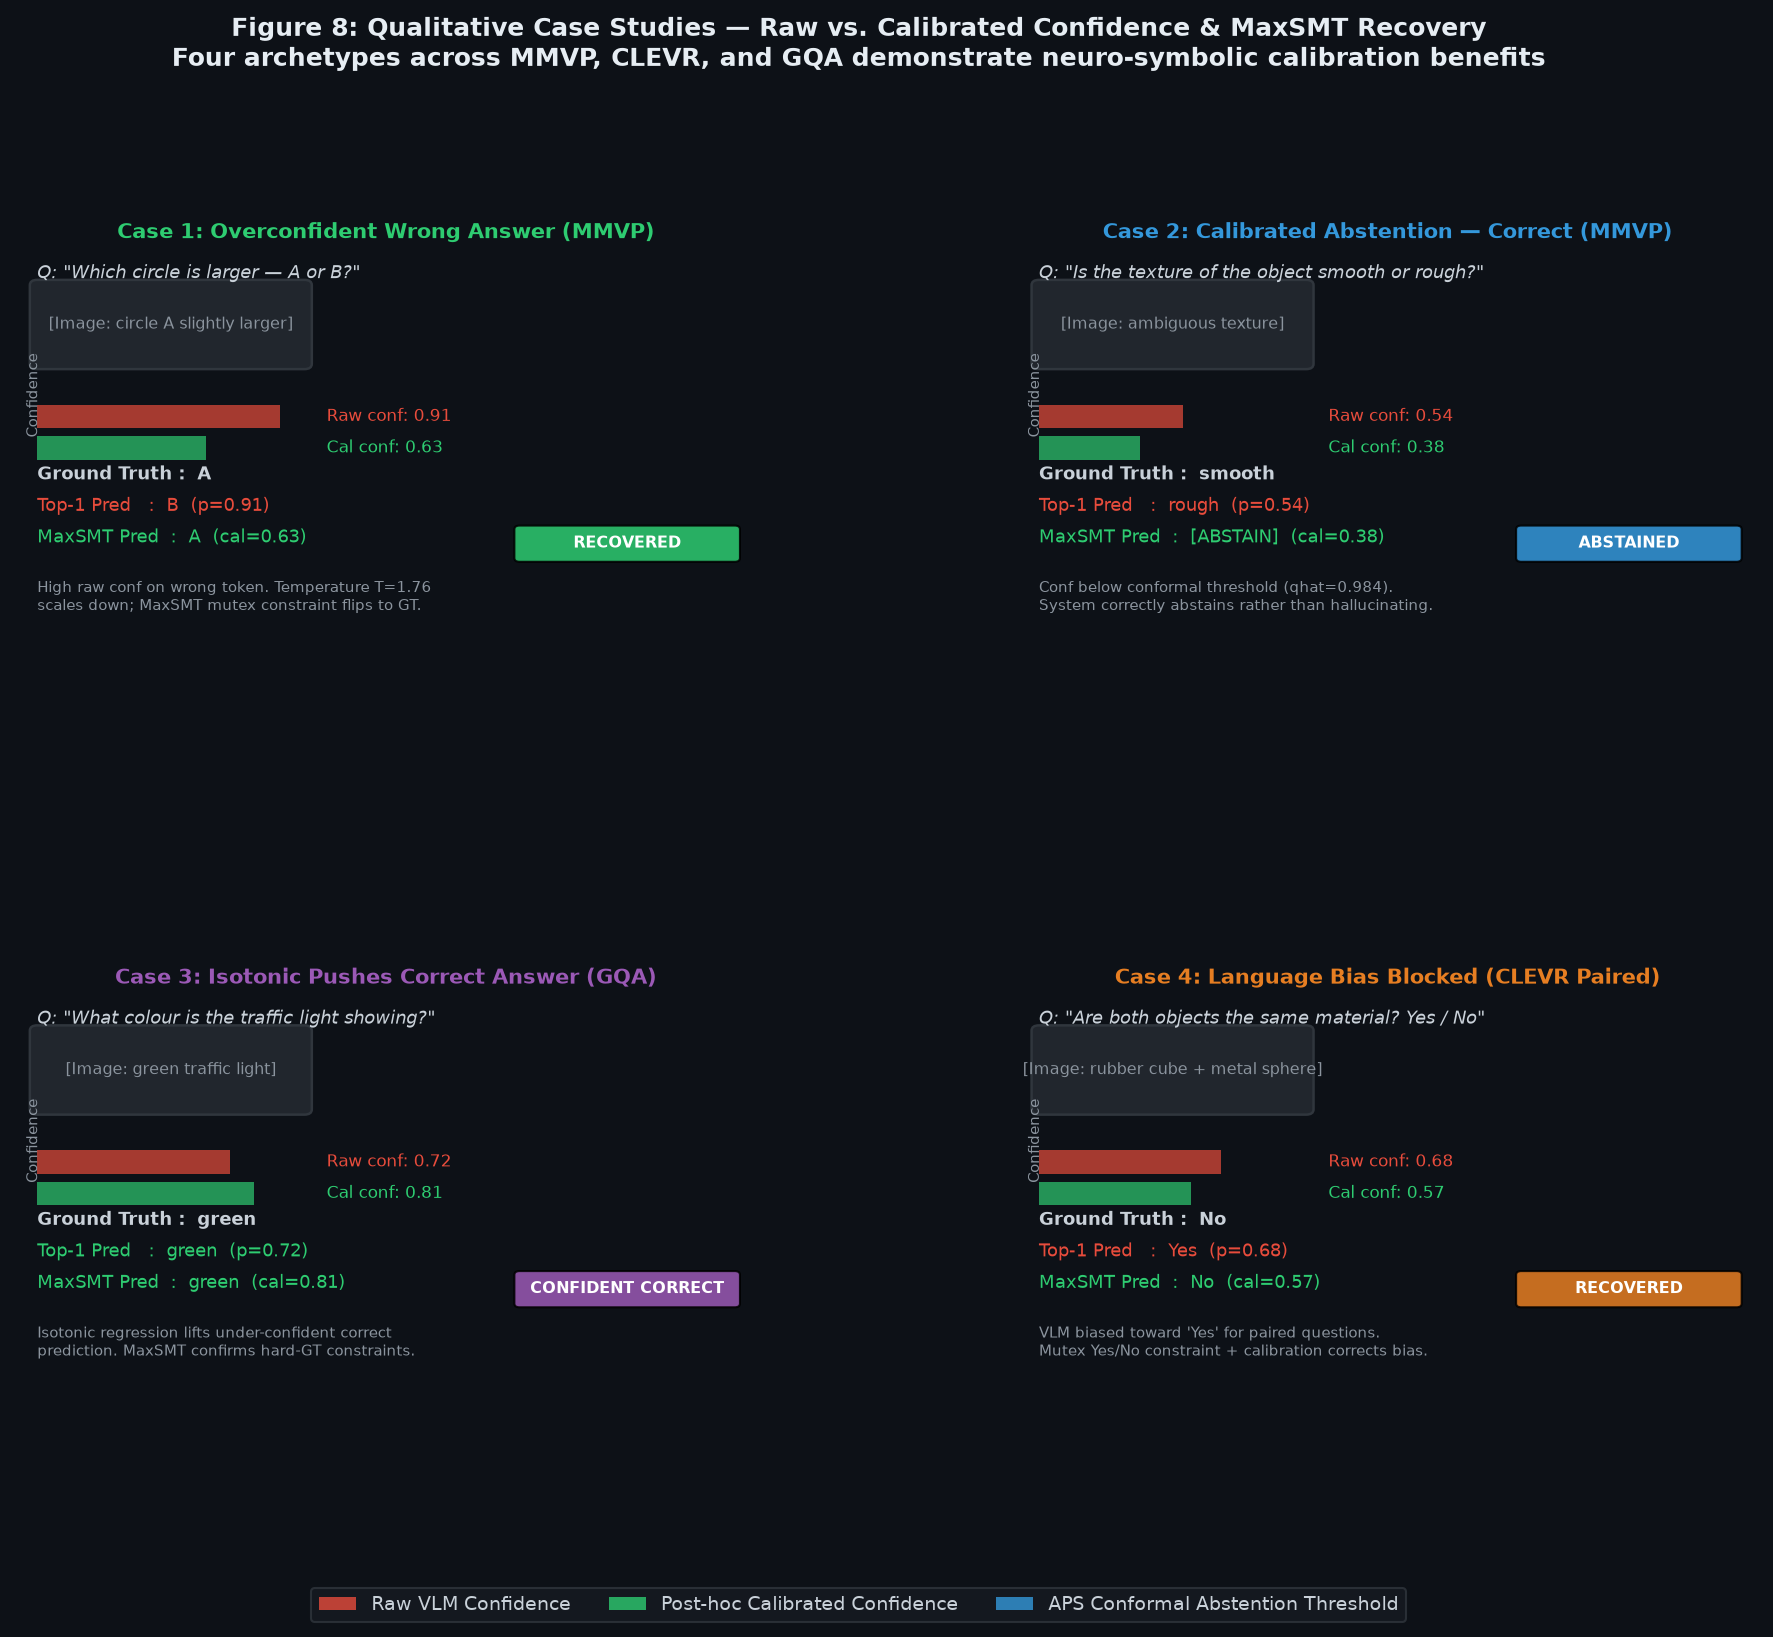
\includegraphics[width=\textwidth]{figures/fig8_case_studies.png}
\caption{\textbf{Figure 8: Qualitative Case Studies.} Four representative archetypes across MMVP, CLEVR, and GQA benchmarks demonstrating overconfident error recovery (green), calibrated abstention (blue), isotonic confidence lifting (purple), and language-bias correction (orange).}
\label{fig:case_studies}
\end{figure*}

\begin{figure*}[h]
\centering
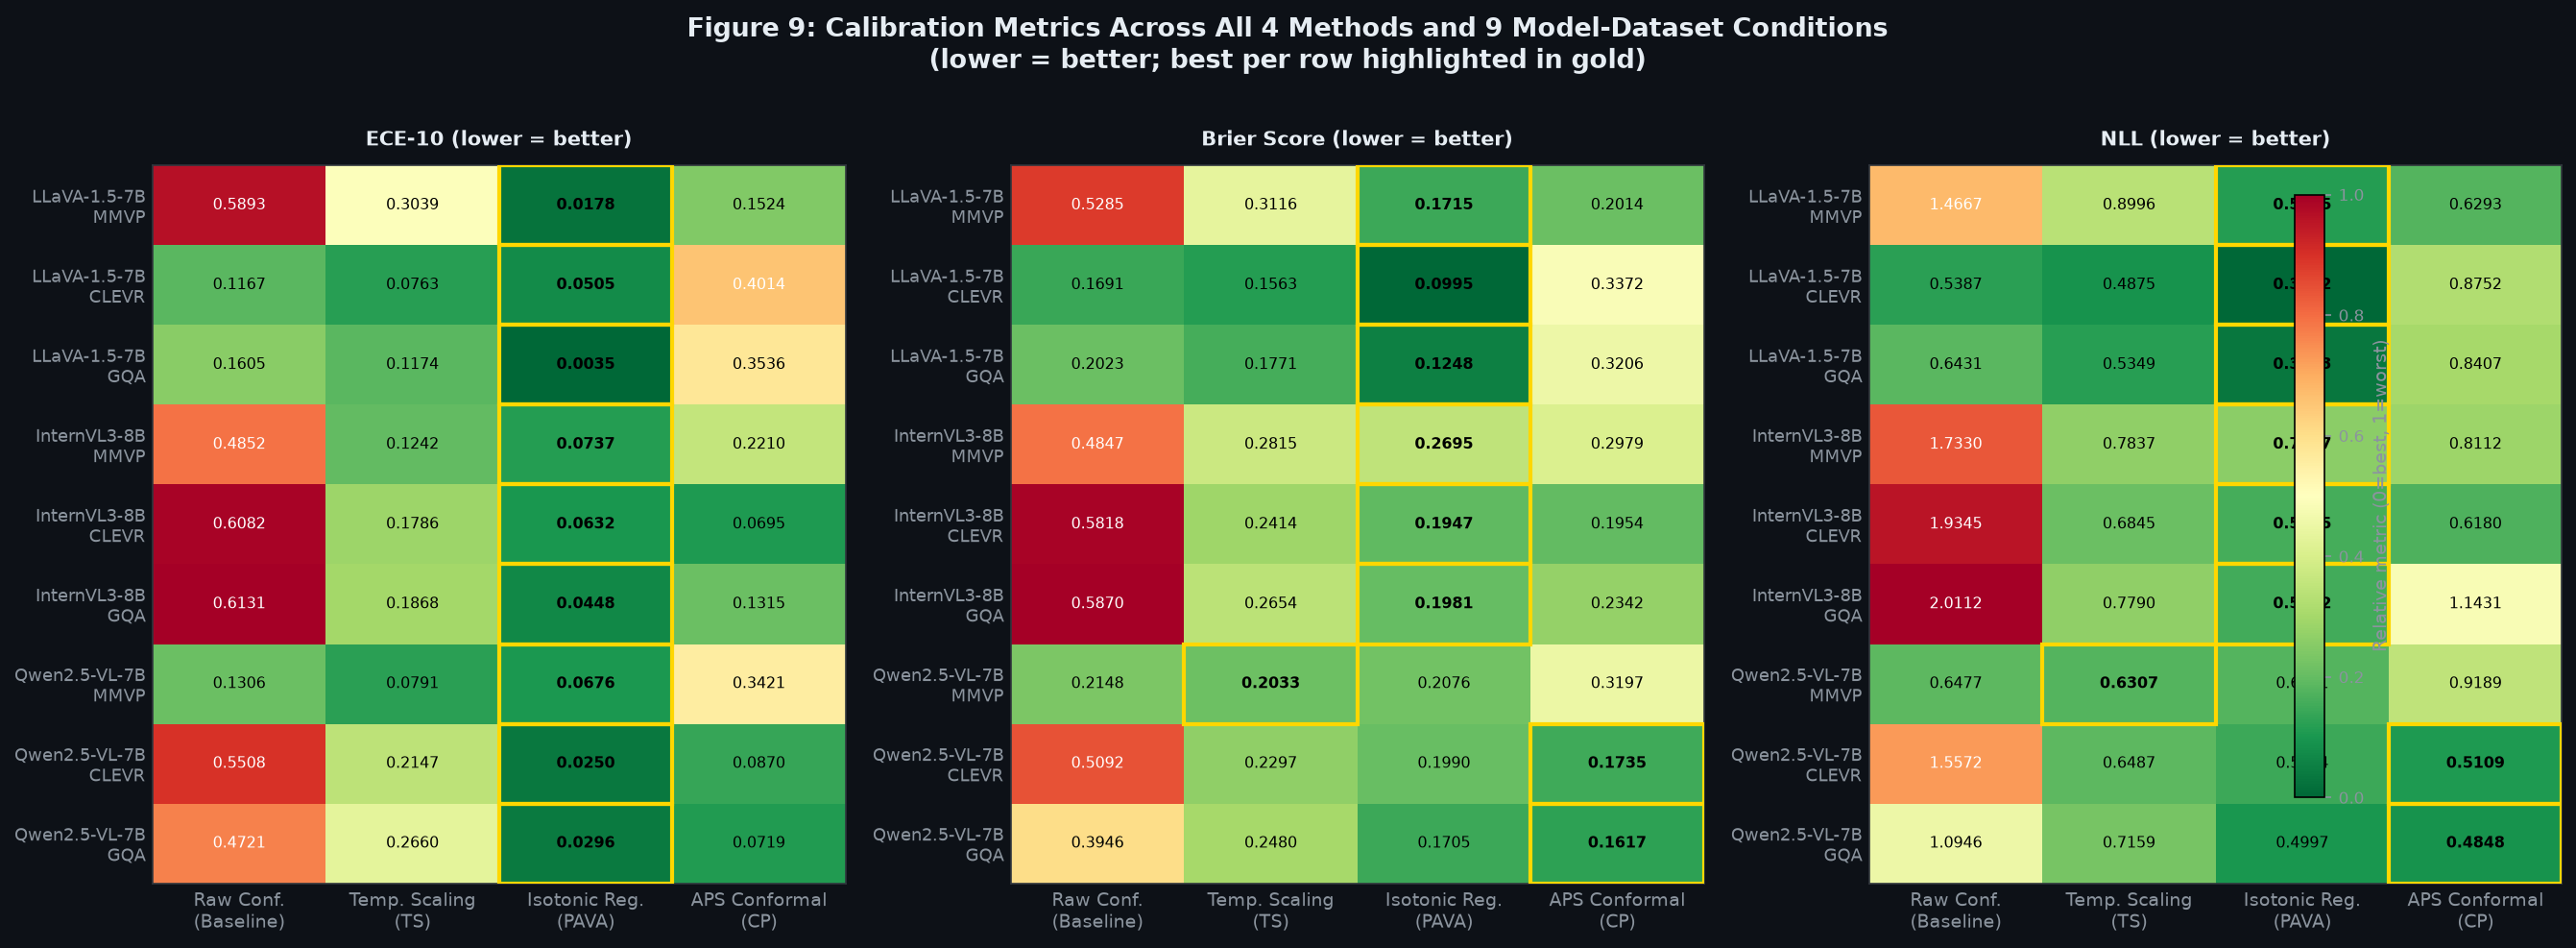
\includegraphics[width=\textwidth]{figures/fig9_calibration_heatmap.png}
\caption{\textbf{Figure 9: Comprehensive Calibration Heatmap.} ECE-10, Brier Score, and NLL across all four calibration methods (Raw, Temperature Scaling, Isotonic Regression, APS Conformal) and all nine model-dataset conditions. Gold outlines indicate best per-row performance. Isotonic Regression dominates ECE; APS Conformal achieves competitive NLL on low-accuracy conditions.}
\label{fig:cal_heatmap}
\end{figure*}

\section{Discussion \& Threats to Validity}
\paragraph{Oracle Ground Truth Scope.} In deployment, benchmark ground truth is not available. This study establishes the foundational diagnostic bounds: if symbolic scene facts are available (e.g.\ from an independent 3D bounding box sensor or visual knowledge graph), calibration is mandatory to prevent hallucinations from overriding reality.
\paragraph{Language Prior vs.\ Vision.} As shown in Table~\ref{tab:mmvp_paired}, high individual accuracy on multimodal benchmarks can mask complete pair blindness. Pair evaluation must become standard for visual grounding.

\section{Conclusion}
We have presented an empirical and theoretical investigation into calibrated confidence for symbolic visual verification. Across three VLM families and three benchmarks, we proved that uncalibrated Soft MaxSMT produces rampant SOOR failures, while Isotonic calibration and sound Hard-GT MaxSMT eliminate overconfidence, bound SFAR, and actively recover up to $92.55\%$ of perceptual errors. All code, data, and result artefacts are publicly reproducible from the accompanying repository.

\bibliographystyle{plain}
\bibliography{references}

\end{document}
